\section{Cauchy-Riemann equations}
The goal of those equations is to check if a function $f$ is differentiable or/and is holomorphic. When we have quite 'easy' function (as seen before) showing that the function is holomorphic by taking the limit is possible. However when function become tedious we will use Cauchy-Riemann questions:
\begin{definition}
Let $w \subseteq \mathbb{C}$ open, $f : w \to \mathbb{C}$ let:
\begin{align*} 
	z = x + iy \mapsto f\left(z\right) =  u\left(x, y\right) + v\left(x, y\right) i
\end{align*}
Be holomorphic. Then, $u, v \in C^{1}\left(w\right)$ (the space of differentiable function $w \subseteq \mathbb{R}^{2} \to \mathbb{R}$) with continuous derivative) and:
\begin{align*} 
	\frac{\partial u}{\partial x} = \frac{\partial v}{\partial y}  \\
	\frac{\partial u}{\partial y}  = -\frac{\partial v}{\partial x} 
\end{align*}
Those equation are called Cauchy-Riemann equations.
\end{definition}
\begin{theoreme}
If the relation:
\begin{align*} 
	\frac{\partial u}{\partial x} = \frac{\partial v}{\partial y}  \\
	\frac{\partial u}{\partial y}  = -\frac{\partial v}{\partial x} 
\end{align*}
holds then $f$ is holomorphic
\end{theoreme}

\begin{parag}{Proof of the direct implication '$\implies$'}
	Suppose that $f$ is holomorphic on $w$, therefore, $\forall z_0 \in w$ we have:
	\begin{align*} 
		f'\left(z_0\right) =  \lim_{z \to z_0} \frac{f\left(z\right) - f\left(z_0\right)}{z - z_0} \mathspace \text{ exists}
	\end{align*}
	We will calculate the limit in two ways. 
\end{parag}
\begin{figure}[!h]
\centering
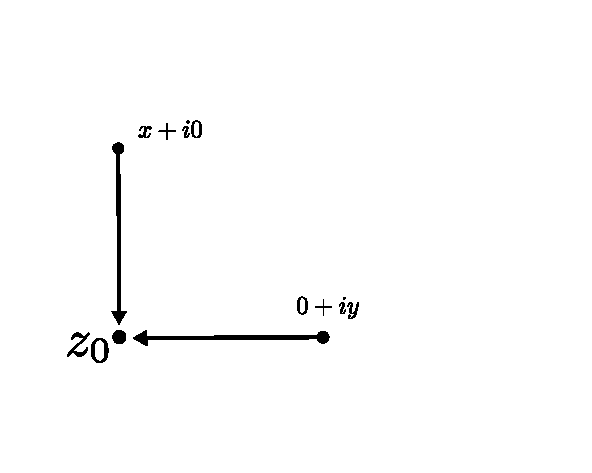
\includegraphics[width=0.5\textwidth]{figure/2026-02-26_1.pdf}
\caption{Two ways of approaching}
\end{figure}
\begin{parag}{$ $}
	First we will approaching $z_0$ from the $x$-direction:
	\begin{align*} 
		f'(z_0) &= \lim_{x \to x_0} \frac{f\left(x + y_0 i\right) - f\left(x_0 + y_0i\right)}{x + y_0i - \left(x_0 + y_0i\right)}\\
				&= \lim_{x \to x_0} \frac{u\left(x, y_0\right) + iv\left(x, y_o\right) - u\left(x_0, y_0\right) - iv\left(x_0, y_0\right)}{x - x_0}\\
				&= \underbrace{\lim_{x \to x_0} \frac{u\left(x, y_0\right) - u\left(x_0, y_0\right)}{x - x_0}}_{= \frac{\partial u}{\partial x}\left(x_0, y_0\right) } + \underbrace{\lim_{x \to x_0}  \frac{v\left(x, y_0\right) - v\left(x_0, y_0\right)}{x - x_0}i}_{= \frac{\partial v}{\partial x} \left(x_0, y_0\right)}
	\end{align*}
	Now we will approach $z_0$ from the $y-$direction:
	\begin{align*} 
		f'\left(z_0\right) &=  \lim_{y \to y_0} \frac{f\left(x_0, yi\right) - f\left(x_0 + y_0i\right)}{x_0 + yi - \left(x_0 + y_0i\right)}\\
						   &= \lim_{y \to y_0} \frac{u\left(x_0, y\right) + iv\left(x_0, y\right) - u\left(x_0, y_0\right) - iv\left(x_0, y_0\right)}{i\left(y - y_0\right)}\\
						   &= \overbrace{\frac{1}{i}}^{= -i} \underbrace{\lim_{y \to y_0} \frac{u\left(x_0, y\right) - u\left(x_0, y_0\right)}{y - y_0}}_{= \frac{\partial u}{\partial y} \left(x_0, y_0\right)} + \frac{i}{i}\underbrace{\lim_{y \to y_0} \frac{v\left(x_0, y\right) - v\left(x_0, y_0\right)}{y - y_0}}_{= \frac{\partial v}{\partial y} \left(x_0, y_0\right)}
	\end{align*}
	By comparing real and imaginary part leads to the Cauchy-Riemann equations. Moreover form this proof, we get explicit expression for $f'\left(z_0\right)$:
	\begin{align*} 
		f' = \frac{\partial u}{\partial x} + \frac{\partial v}{\partial x} i =  \frac{\partial v}{\partial y}  - \frac{\partial u}{\partial y} i
	\end{align*}
\end{parag}


\begin{parag}{Example}
    $f : \mathbb{C}^{\ast} \to \mathbb{C}$, $f\left(z\right) = \frac{1}{z} $
	\begin{align*} 
		f\left(z\right) &= \frac{\overline{z}}{\left\|z\right\|^2}\\
						&= \frac{x}{x^2 + y^2} - \frac{y}{x^2 + y^2}i\\
						&= u\left(x, y\right) + v\left(x, y\right)i
	\end{align*}
	Now we will compute the Cauchy-Riemann equations:
	\begin{align*} 
		\frac{\partial u}{\partial x} = \frac{x^2 + y^2 - 2x^2}{\left(x^2 + y^2\right)^2} \mathspace \mathspace \frac{\partial v}{\partial x} = \frac{2xy}{\left(x^2 + y^2\right)^2}
	\end{align*}
	\begin{align*} 
		\frac{\partial u}{\partial y} = -\frac{2xy}{\left(x^2 + y^2\right)^2} \mathspace \mathspace \frac{\partial v}{\partial y} = \frac{-\left(x^2 + y^2\right) + 2y^2}{\left(x^2 + y^2\right)^2}
	\end{align*}
	We therefore the Cauchy-Riemann equations satisfied and:
	\begin{align*} 
		f' &= \frac{\partial u}{\partial x}  + \frac{\partial v}{\partial x} i \\
			&= \frac{y^2 - x^2}{\left(x^2 + y^2\right)^2} + \frac{2xy}{\left(x^2 + y^2\right)^2}i
	\end{align*}
	Indeed, this coincides with $-\frac{1}{z^2}$ (computation).
\end{parag}

\begin{parag}{Example}
	The last example will be: $f\left(z\right) =  e^{z}$ let us massage our function:
	\begin{align*} 
		f\left(z\right) &= e^{x + yi} = e^{x}e^{yi}\\
						&= e^{x}\cos y + e^{x}\sin \left(y\right) i\\
						&= u\left(x, y\right) + iv\left(x, y\right)
	\end{align*}
	Not let us compute the Cauchy-Riemann equations:
	\begin{align*} 
		\frac{\partial u}{\partial x} &= e^{x}\cos y \mathspace \mathspace \frac{\partial v}{\partial x} = e^{x}\sin y \\
		\frac{\partial u}{\partial y} &= -e^{x}\sin y \mathspace \mathspace \frac{\partial v}{\partial y} = e^{x}\cos y
	\end{align*}
	As we can see that equation holds which implies that our function $f$ is holomorphic.\\
	$ $\\
	Moreover, the derivative of our function is given as:
	\begin{align*} 
		f' = \frac{\partial u}{\partial x} + i \frac{\partial v}{\partial x} = e^{x}\cos y + ie^{x}\sin y = e^{z}
	\end{align*}
\end{parag}

\subsection{Rules for differentiation}
\begin{theoreme}
Let $f, g: w \to \mathbb{C}$ holomorphic. Then:
\begin{align*} 
	\left(f + g\right)' &= f' + g'\\
	\left(fg\right)' &= f'g + fg' \mathspace \mathspace\mathspace \mathspace \mathspace \text{Leibniz rule}\\
	\left(\frac{f}{g}\right)' &= \frac{f'g - fg'}{g^2} \mathspace \mathspace \mathspace g \neq 0
\end{align*}
If the image of $g$ is inside of $w$:
\begin{align*} 
	\left(f \circ g\right)'\left(z\right) =  f'\left(g\left(z\right)\right) \cdot g'\left(z\right)\mathspace \mathspace\mathspace \mathspace \mathspace \text{chain rule}
\end{align*}
\end{theoreme}
All of these relations can be shown exactly as in the real case, we will do $\left(fg\right)'\left(z_0\right)$. First let us use the definition of the derivative:
\begin{align*} 
	\left(fg\right)'\left(z_0\right) &= \lim_{z \to z_0} \frac{f\left(z\right)g\left(z\right) - f\left(z_0\right)g\left(z_0\right)}{z - z_0}\\
									 &= \lim_{z \to z_0} \frac{f\left(z\right)g\left(z\right) - f\left(z_0\right)g\left(z\right) + f\left(z_0\right)g\left(z\right) - f\left(z_0\right)g\left(z_0\right)}{z - z_0}\\
									 &= \lim_{z \to z_0} \frac{f\left(z\right) - f\left(z_0\right)}{z - z_0}g\left(z\right) + f\left(z_0\right)\frac{g\left(z\right) - g\left(z_0\right)}{z - z_0}\\
									 &= f'\left(z_0\right)g\left(z_0\right) + f\left(z_0\right)g'\left(z_0\right)
\end{align*}
With these rules and previous examples, it follows the usual formulas for differentiation of polynomial, trigonometric functions, etc...
\begin{align*} 
	\left(z^{k}\right)' &=  kz^{k-1}\\
	\left(\cos z\right)' &= -\sin z\\
	\left(\sin z\right)' &= \cos z
\end{align*}
\begin{parag}{Geometric interpretation of Cauchy-Riemann equations}
    Let's fix $f : \mathbb{C} \to \mathbb{C}$ holomorphic, and view it as a function $f : \mathbb{R}^{2} \to \mathbb{R}^{2}$. Geometrically the Jacobian matrix:
	\begin{align*} Df = \begin{pmatrix} \frac{\partial u}{\partial x}  & \frac{\partial v}{\partial x}  \\ \frac{\partial u}{\partial y}  & \frac{\partial v}{\partial y}  \end{pmatrix}  \end{align*}
	tells us how $f$ acts on 'infinitesimal rectangles'/ disturb volume.

\end{parag}
\begin{figure}[!h]
\centering
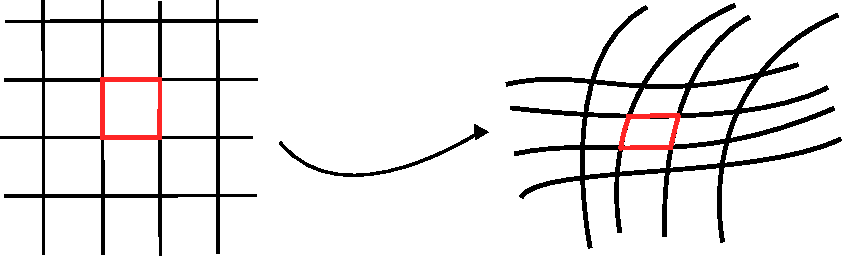
\includegraphics[width=1.0\textwidth]{figure/2026-02-26_2.pdf}
\caption{Transformation of the Jacobian matrix}
\end{figure}
A very specific deformation happens for holomorphic functions. In fact, the Cauchy-Riemann equations imply that the Jacobian is in the form of:
\begin{align*} 
	Df &= \begin{pmatrix} a & -b \\ b & a \end{pmatrix} \\
	   &= \sqrt{a^2 + b^2}\underbrace{\begin{pmatrix} \frac{a}{\sqrt{a^2 + b^2}} & -\frac{b}{\sqrt{a^2 + b^2}} \\ \frac{b}{\sqrt{a^2 + b^2}} & \frac{a}{\sqrt{a^2 + b^2}} \end{pmatrix} }_{\text{rotation matrix}}
\end{align*}
Recall that a  rotation matrix is in the form of:
\begin{align*} 
	\begin{pmatrix} \cos \theta & \sin \theta \\ -\sin \theta & \cos \theta \end{pmatrix} 
\end{align*}
Hence we have that $Dg =  \lambda \cdot $rotation! Therefore, infinitesimal square is mapped to a square.
\subsection{Complex logarithm}
First let us recall what the principal argument is. For $z \neq 0$ we have that $-\pi < $ Arg $z \leq \pi$

\begin{center}
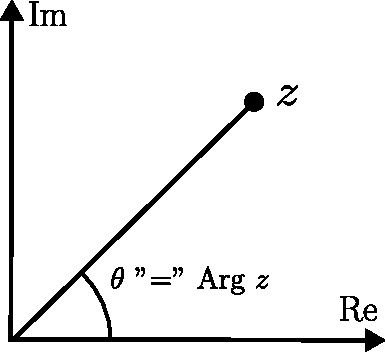
\includegraphics[width=0.3\textwidth]{figure/2026-02-27.pdf}
\end{center}
It can be computed by:
\begin{align*} 
	\text{Arg}z =  \begin{cases}
		\arctan \frac{y}{x} \mathspace \mathspace \mathspace &\text{ if } x > 0\\
		\frac{\pi}{2} &\text{ if } x = 0, y > 0\\
		\pi + \arctan \frac{y}{x} &\text{ if } x < 0, y \geq 0\\
		-\frac{\pi}{2} &\text{ if }x = 0, y < 0\\
		-\pi + \arctan \frac{y}{x} &\text{ if } x < 0, y < 0
	\end{cases}
\end{align*}
Arg is (defined yet) \important{discontinuous} on the negative real axis, it jumps from $\pi$ to $-\pi$ across the negative real axis.\\
$ $\\
Okay this is nice but why are we even talking about this here in the first case, we are trying to define the logarithm for complex number. How de we define complex logarithm? First what does it do? It is the inverse of the exponential meaning that we should have $\log e^{z} =  z$. If we expand $z$ into Cartesian form, $\log\left(e^{x + iy}\right) = x + iy$.\\
$ $\\
If $\log z =  x + iy$ then we should have $z = e^{x + iy} = e^{x}e^{yi}$. By polar coordinate, we can also define $z$ as:

\begin{align*} 
	z = \underbrace{\left\|z\right\|}_{= e^{x}}\underbrace{e^{i\text{Arg}z}}_{= e^{iy} }
	\end{align*}
	\begin{framedremark}
	We are allowed to do so because $z = e^{x + iy}$. In general we don't have $y =  $Arg $z$. Now we have something that could be put into the $\log$:
	\end{framedremark}
\begin{definition}
	We define:
	\begin{align*} 
		lg z =  lg \left\|z\right\| + i \text{Arg} z
	\end{align*}
	Complex logarithm, more precisely the principal branch of complex algorithm
\end{definition}
\begin{framedremark}
\begin{itemize}
    \item $\log z$ is not defined at $z= 0$
    \item $\log z$ is discontinuous on the negative real axis
\end{itemize}
More precisely, computing $\log z$ for $z =  x + iy$ with $x > 0$:
\begin{align*} 
	\log z &=  \log \sqrt{x^2 + y^2} + i \arctan \frac{y}{x}\\
		   &= u\left(x, y\right) + iu\left(x, y\right)
\end{align*}
It is easy to verify that $\log$ is holomorphic on $\mathbb{C} \setminus \left\{Im = 0, Re \leq 0\right\}$ and $\left(\log z\right)' = \frac{1}{z}$
\end{framedremark}
\begin{parag}{logarithm rules}
    
\begin{align*}
	\log\left(z_1z_2\right) &= \log\left(z_1\right) + \log\left(z_2\right)\\
	\log\left(z^{\gamma}\right) &= \gamma\log \left(z\right) \mathspace \mathspace \gamma \in \mathbb{C}
\end{align*}
\end{parag}
\begin{parag}{Example}
    If $z_1 =  z_2 =  -1$ then $\log z_1 =  \log z_2 =  i\pi$. (since $e^{i\pi}= -1$). Yet we have that $\log\left(z_1z_2\right) =  0 \neq\log\left(z_1\right) + \log \left(z_2\right)$. Similarly 
	\begin{align*} 
		\log \left(z_1^2\right) \neq 2\log\left(z_1\right) 
	\end{align*}
		However these rules remain true up to $2\pi i\mathbb{Z}$:
		\begin{align*} 
			\log\left(z_1z_2\right) - \log z_1 - \log z_2 \in 2\pi i \mathbb{Z} \\
			\log\left(z^{\gamma}\right) - \gamma \log \left(z\right) \in 2\pi i \mathbb{Z}
		\end{align*}
\end{parag}






